\documentclass[12pt]{article}

% Paquetes
\usepackage[spanish]{babel}
\usepackage[utf8]{inputenc}
\usepackage[T1]{fontenc}
\usepackage{geometry}
\usepackage{graphicx}
\usepackage{listings}
\usepackage{xcolor}

\geometry{a4paper, margin=2.5cm}

% Configuracion codigo Octave
\lstset{
    language=Octave,
    basicstyle=\ttfamily\small,
    keywordstyle=\color{blue},
    stringstyle=\color{red},
    commentstyle=\color{green!60!black},
    numbers=left,
    numberstyle=\tiny,
    frame=single,
    breaklines=true
}

\begin{document}

% ---------------- CARATULA ----------------
\begin{titlepage}
\centering

{\large UNIVERSIDAD MAYOR DE SAN ANDRES \\
FACULTAD DE CIENCIAS PURAS Y NATURALES \\
CARRERA DE MATEMATICA \\}

\vspace{2cm}

{\Large \textbf{ANALISIS E IMPLEMENTACION DE NUMEROS PRIMOS EN OCTAVE}}

\vspace{2cm}

\textbf{Materia:} Computacion Cientifica \\
\textbf{Sigla:} Computacion 117 \\

\vspace{2cm}

\textbf{Estudiante:} Miguel ............................................. \\
\textbf{Docente:} ............................................. \\

\vfill

La Paz - Bolivia \\
2026

\end{titlepage}

% ---------------- INDICE ----------------
\tableofcontents
\newpage

% ---------------- INTRODUCCION ----------------
\section{Introduccion}

Los numeros primos constituyen uno de los conceptos mas importantes en la matematica discreta. Su estudio ha sido fundamental en el desarrollo de diversas areas como la teoria de numeros, la criptografia y la computacion.

En este trabajo se desarrolla un programa en Octave que permite verificar si un numero es primo y generar una cantidad determinada de numeros primos, utilizando estructuras basicas de programacion.

% ---------------- FUNDAMENTO TEORICO ----------------
\section{Fundamento Teorico}

Un numero primo es aquel numero natural mayor que 1 que tiene exactamente dos divisores positivos: el 1 y el mismo numero.

\subsection{Propiedades de los numeros primos}
\begin{itemize}
\item El numero 2 es el unico numero primo par.
\item Todo numero compuesto puede expresarse como producto de numeros primos.
\item Los numeros primos son infinitos (demostrado por Euclides).
\end{itemize}

\subsection{Importancia en computacion}
Los numeros primos son esenciales en algoritmos criptograficos como RSA, donde se utilizan para generar claves seguras.

% ---------------- CODIGO ----------------
\section{Codigo Fuente}

\begin{lstlisting}
clc;

fprintf('============================\n');
fprintf('   MENU DE NUMEROS PRIMOS   \n');
fprintf('============================\n');
fprintf('1. Verificar si un numero es primo\n');
fprintf('2. Generar N numeros primos\n');
fprintf('============================\n');

op = input('Elija una opcion (1 o 2): ');

if op == 1
    n = input('Ingrese un numero: ');

    if n <= 1
        fprintf('El numero NO es primo\n');
    else
        primo = 1;

        for i = 2:n-1
            if mod(n,i) == 0
                primo = 0;
            end
        end

        if primo == 1
            fprintf('El numero %d es primo\n', n);
        else
            fprintf('El numero %d NO es primo\n', n);
        end
    end

elseif op == 2
    n = input('Ingrese cantidad de primos: ');

    cont = 0;
    num = 2;

    while cont < n
        primo = 1;

        for i = 2:num-1
            if mod(num,i) == 0
                primo = 0;
            end
        end

        if primo == 1
            fprintf('%d ', num);
            cont = cont + 1;
        end

        num = num + 1;
    end

    fprintf('\n');

else
    fprintf('Opcion no valida\n');
end
\end{lstlisting}

% ---------------- EJECUCION ----------------
\section{Ejecucion del Programa}

\begin{figure}[h]
\centering
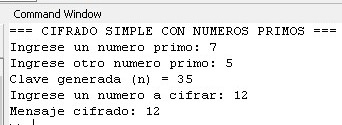
\includegraphics[width=0.8\textwidth]{ejemplo1.jpg}
\caption{Ejecucion del programa en Octave}
\end{figure}

% ---------------- EXPLICACION ----------------
\section{Explicacion de la Corrida}

El programa presenta un menu interactivo donde el usuario selecciona la operacion deseada. Dependiendo de la opcion, el sistema evalua si un numero es primo mediante divisibilidad o genera una secuencia de numeros primos.

% ---------------- PROBLEMAS ADICIONALES ----------------
\section{Problemas y Aplicaciones Adicionales}

Los numeros primos permiten resolver diversos problemas computacionales y matematicos:

\subsection{Ejercicio 1: Factorizacion prima}
Descomponer un numero en sus factores primos. Ejemplo: 20 = 2 x 2 x 5.

\subsection{Ejercicio 2: Encontrar el siguiente primo}
Dado un numero, encontrar el siguiente numero primo mayor.

\subsection{Ejercicio 3: Primos gemelos}
Identificar pares de numeros primos cuya diferencia es 2, como (3,5) o (11,13).

\subsection{Ejercicio 4: Criba de Eratostenes}
Metodo eficiente para encontrar todos los numeros primos hasta un limite dado.

\subsection{Ejercicio 5: Aplicacion en criptografia}
Uso de numeros primos grandes para generar claves seguras en sistemas de cifrado.

% ---------------- CONCLUSIONES ----------------
\section{Conclusiones}

Se desarrollo un programa funcional en Octave que permite trabajar con numeros primos mediante algoritmos basicos. Este tipo de implementaciones fortalece el aprendizaje de estructuras de control y logica computacional.

% ---------------- RECOMENDACIONES ----------------
\section{Recomendaciones}

Se recomienda mejorar la eficiencia del algoritmo mediante optimizaciones como la reduccion del rango de division o el uso de estructuras de control adicionales.

% ---------------- BIBLIOGRAFIA ----------------
\section{Bibliografia}

\begin{itemize}
\item Rosen, K. (2012). \textit{Matematica Discreta y sus Aplicaciones}.
\item Stallings, W. (2017). \textit{Criptografia y Seguridad en Redes}.
\item Apostol, T. (1976). \textit{Introduccion a la Teoria de Numeros}.
\item Documentacion oficial de GNU Octave: https://www.octave.org
\end{itemize}

\end{document}